\documentclass{article}
\usepackage[utf8]{inputenc}

\title{Online voting: measure of privacy and verifiability}
\author{boire.sebastien }
\date{November 2020}

\usepackage{natbib}
\usepackage{graphicx}
\usepackage{amsmath}
\usepackage{amssymb}

\begin{document}

\maketitle


\section{Definitions of privacy and verifiability}

\subsection{Quantifying information on a vote}

If we have access to some partial information on a vote, we want to measure the mount of information we can get from it. From a message mes, we define a function quantifying the information on the message as:

$Info(mes)=\dfrac{\text{number of possible votes coherent with mes}}{total number of possible votes}$

This definition can be applied to the vote of one user, with a receipt providing partial information on the vote, but also on an entire election, with mes being all the public information we have access to.


\subsection{Privacy}

Privacy is the amount of money required to buy one vote, taking into account the probability that the vote was correctly bought. For instance, if 10€ are given to any person who has a proof such that "I voted for candidate A or candidate B", with candidate A being the one that we want to buy, then privacy amounts to 20€. (This holds true if the voter cannot choose A and B appearing in his proof, but only chooses who he votes for).


$privacy=\dfrac{\text{cost to change one vote}}{\text{probability that the vote was performed according to the attacker's will}}$


\subsection{Verifiability}

The election can be verified using all the public information on the votes. We define verifiability as:

$Verifiability=Info(\text{all public receipts})*\text{level of verification}$

The level of verification is the probability with which the verification confirms the result of the election.


\section{First scheme: public storage of a subset of possible vote values}

\subsection{Description}

We consider an election with candidates $C_1, ..., C_K$. Voter V votes for $C_i$, and the value of the vote is stored encrypted so that it can be counted, verified by V, and secret. In addition, (k-1) other candidates are chosen at random, and a public ticket is produced: "Voter V voted for $C_{i_1}$ or $C_{i_2}$ or ... or $C_{i_k}$.", with one of the $C_{i_j}$ being $C_i$, the correct value.

\subsection{Evaluation of verifiability}

We note $X^i_j$ the binary variable corresponding to "Does voter j voted for candidate i?". Then:

$Y_\alpha^i=X^i_1+...+X^i_\alpha$ is a binomial variable following $\mathcal{B}(\alpha, p_i)$, with $p_i$ probability of vote for candidate i.

In a similar way, we note $\tilde{X}^i_j$ the binary variable corresponding to "Does the public vote of voter j contains candidate i as a possible vote?".

$\tilde{Y}_\alpha^i=\tilde{X}^i_1+...+\tilde{X}^i_\alpha$ is a binomial variable following $\mathcal{B}(\alpha, \tilde{p}_i)$, with $\tilde{p}_i$ probability that candidate i is in a public vote.

We have:

$\tilde{p}_i=p_i+(1-p_i)*\frac{k-1}{K-1}$


We use Bienayme-Tchebychev inequality on $\tilde{Y}_\alpha^i$:

$ \mathbb{P}(|\dfrac{\tilde{Y}^i_\alpha-\alpha*\tilde{p}_i}{\alpha}| > x )  \leqslant \dfrac{\tilde{p}_i(1-\tilde{p}_i)}{\alpha x^2}$


Using the public votes of $\alpha$ voters, we can compare the scores we obtain for each candidate to the global results of the election, and measure whether the difference is likely or not. This provides a measure of verifiability (we just need to choose a level of verification with the term $\dfrac{\tilde{p}_i(1-\tilde{p}_i)}{\alpha x^2}$).


\subsection{Evaluation of privacy}

Privacy can be defined in multiple ways. Here, we will measure the entropy on one vote, as the amount of unknown information to an attacker to know one vote.

$Privacy=H(vote)=-\sum\limits_{c \in candidates} p(c)log_2(p(c))=log_2(k)$

In this, we do not take into account that each candidate has a probability $p_i$ of being the real value of the vote (to simplify calculations). This corresponds to the situation where each candidate obtains as much vote as any other.


\section{Second scheme: public storage of the votes under probabilistic value}


\subsection{Description}

The election is in the same configuration as in the previous section. However, before the the voter chooses who he votes for, he sees a set of random variables appearing on the screen: $R_1, ..., R_K$. They all follow a Gaussian law, with $R_1$ following a $\mathcal{N}(\mu, \sigma^2)$, and all the other $R_i$ following a $\mathcal{N}(\frac{1-\mu}{K}, \sigma^2)$. Then, the voter chooses who he votes for, and the variables $R_i$ are rotated so that $R_1$ is associated to the candidate chosen by the voter. The values of the $R_i$ are then made public. 

$\mu$ is chosen such that $\mu > \frac{1-\mu}{K}$, so that on average we can distinguish the correct candidate. The bigger the difference, the easier it is to identify the real value of the vote. In addition, $\sigma$ quantifies the randomness of the values of $R_i$, and also takes part in how easy it is to identify the real value of a vote.

\bigbreak

This structure allows the voter to be sure that he is not duped on the value of his public vote, since the random variables $R_i$ are evaluated before the voter enters his vote.

\bigbreak

For simplicity, $R_1$ is chosen to be $1-(R_2+\cdots+R_K)$ such that the sum results in 1.


\subsection{Privacy evaluation}

An attacker who wants to buy votes will rely on the public receipt of the vote, which only contains partial information. Therefore, the attacker will pay an amount proportional to $R_j$.

We suppose that the voter wants to vote for $C_1$, and the attacker wants the voter to vote for $C_j$, $j\neq 1$. The attacker will consider that the user voted for the candidate associated to the highest of the $R_i$s. We need to measure the frequency that the highest of the $R_i$s is associated to $C_1$, revealing the correct vote. The parameters that can be modified are:
\begin{itemize}
    \item $\epsilon$: this defines the mean for the distribution of $R_1$, as $\mu + \epsilon$. $\epsilon$ determines how confident the verification can be.
    \item $\sigma$: the highest the sigma, the more dense the distributions. $\sigma$ determines how many votes are necessary for the result of the verification to be trustworthy.
\end{itemize}

We generate random sets of $R_1, \cdots, R_K$, and measure the probability that each one is associated to both distribution. We note $D_1$ the distribution of $R_1$ (correct value of the vote), and $D_2$ the distribution of the incorrect values of the vote (for $R_2, \cdots, R_K$).

We have:

$\mathbb{P}(R_i\text{ follows }D_1 | \text{1 of the Rs follows }D_1)=\dfrac{\mathbb{P}(R_i\sim D_1)\mathb{P}(R_1 \sim D_2)\cdots \mathbb{P}(R_K \sim D_2)}{\sum\limits_{j=1}^{K}\mathbb{P}(R_j\sim D_1)\mathb{P}(R_1 \sim D_2)\cdots \mathbb{P}(R_K \sim D_2)}$

We count the number of times that $\mathbb{P}(R_i\text{ follows }D_1 | \text{1 of the Rs follows }D_1)$ is maximum for i=1 as the number of times the correct vote of the user is revealed to the attacker. Ideally, it should happen 1/K times.

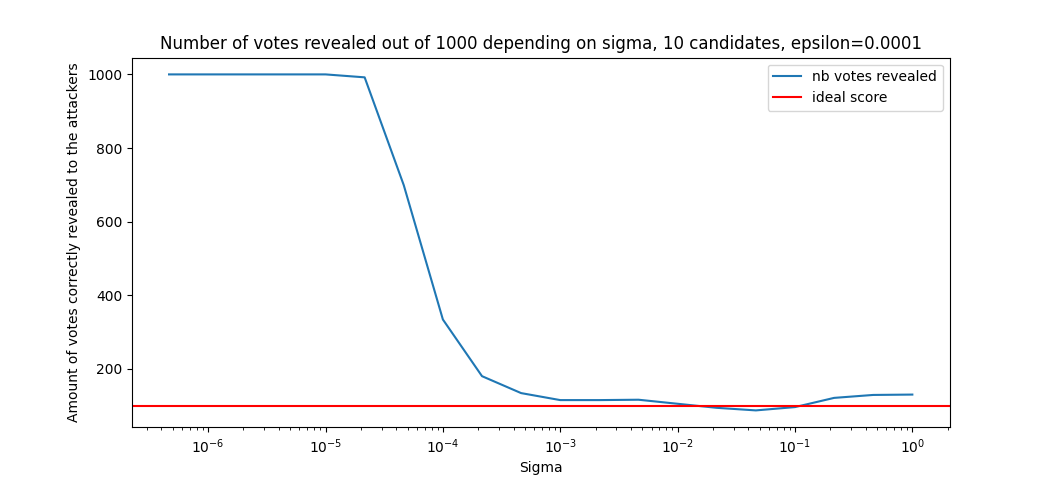
\includegraphics[scale=0.5]{distribution_proba/influence_sigma.png}
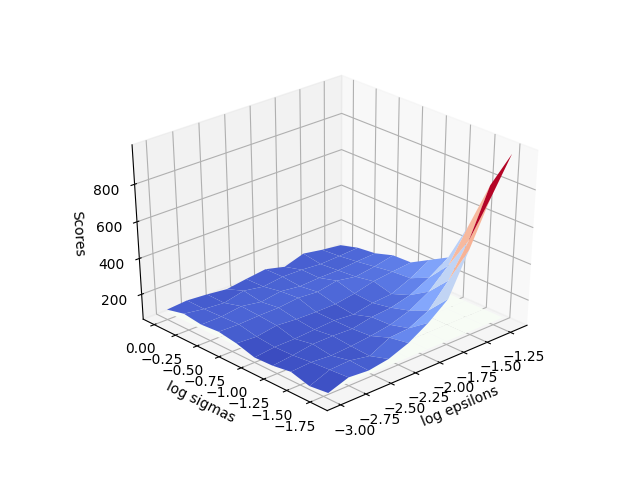
\includegraphics[scale=0.8]{distribution_proba/influence_sigma_epsilon.png}

\subsection{Verifiability evaluation}



\subsection{Privacy evaluation}


\section{Third scheme: Privacy of the votes depending on subgroups of the voting population}

\end{document}
 
